\subsection{System Model}
\begin{figure}[H]
  \subsubsection{Schedule new Job}
  \centering
  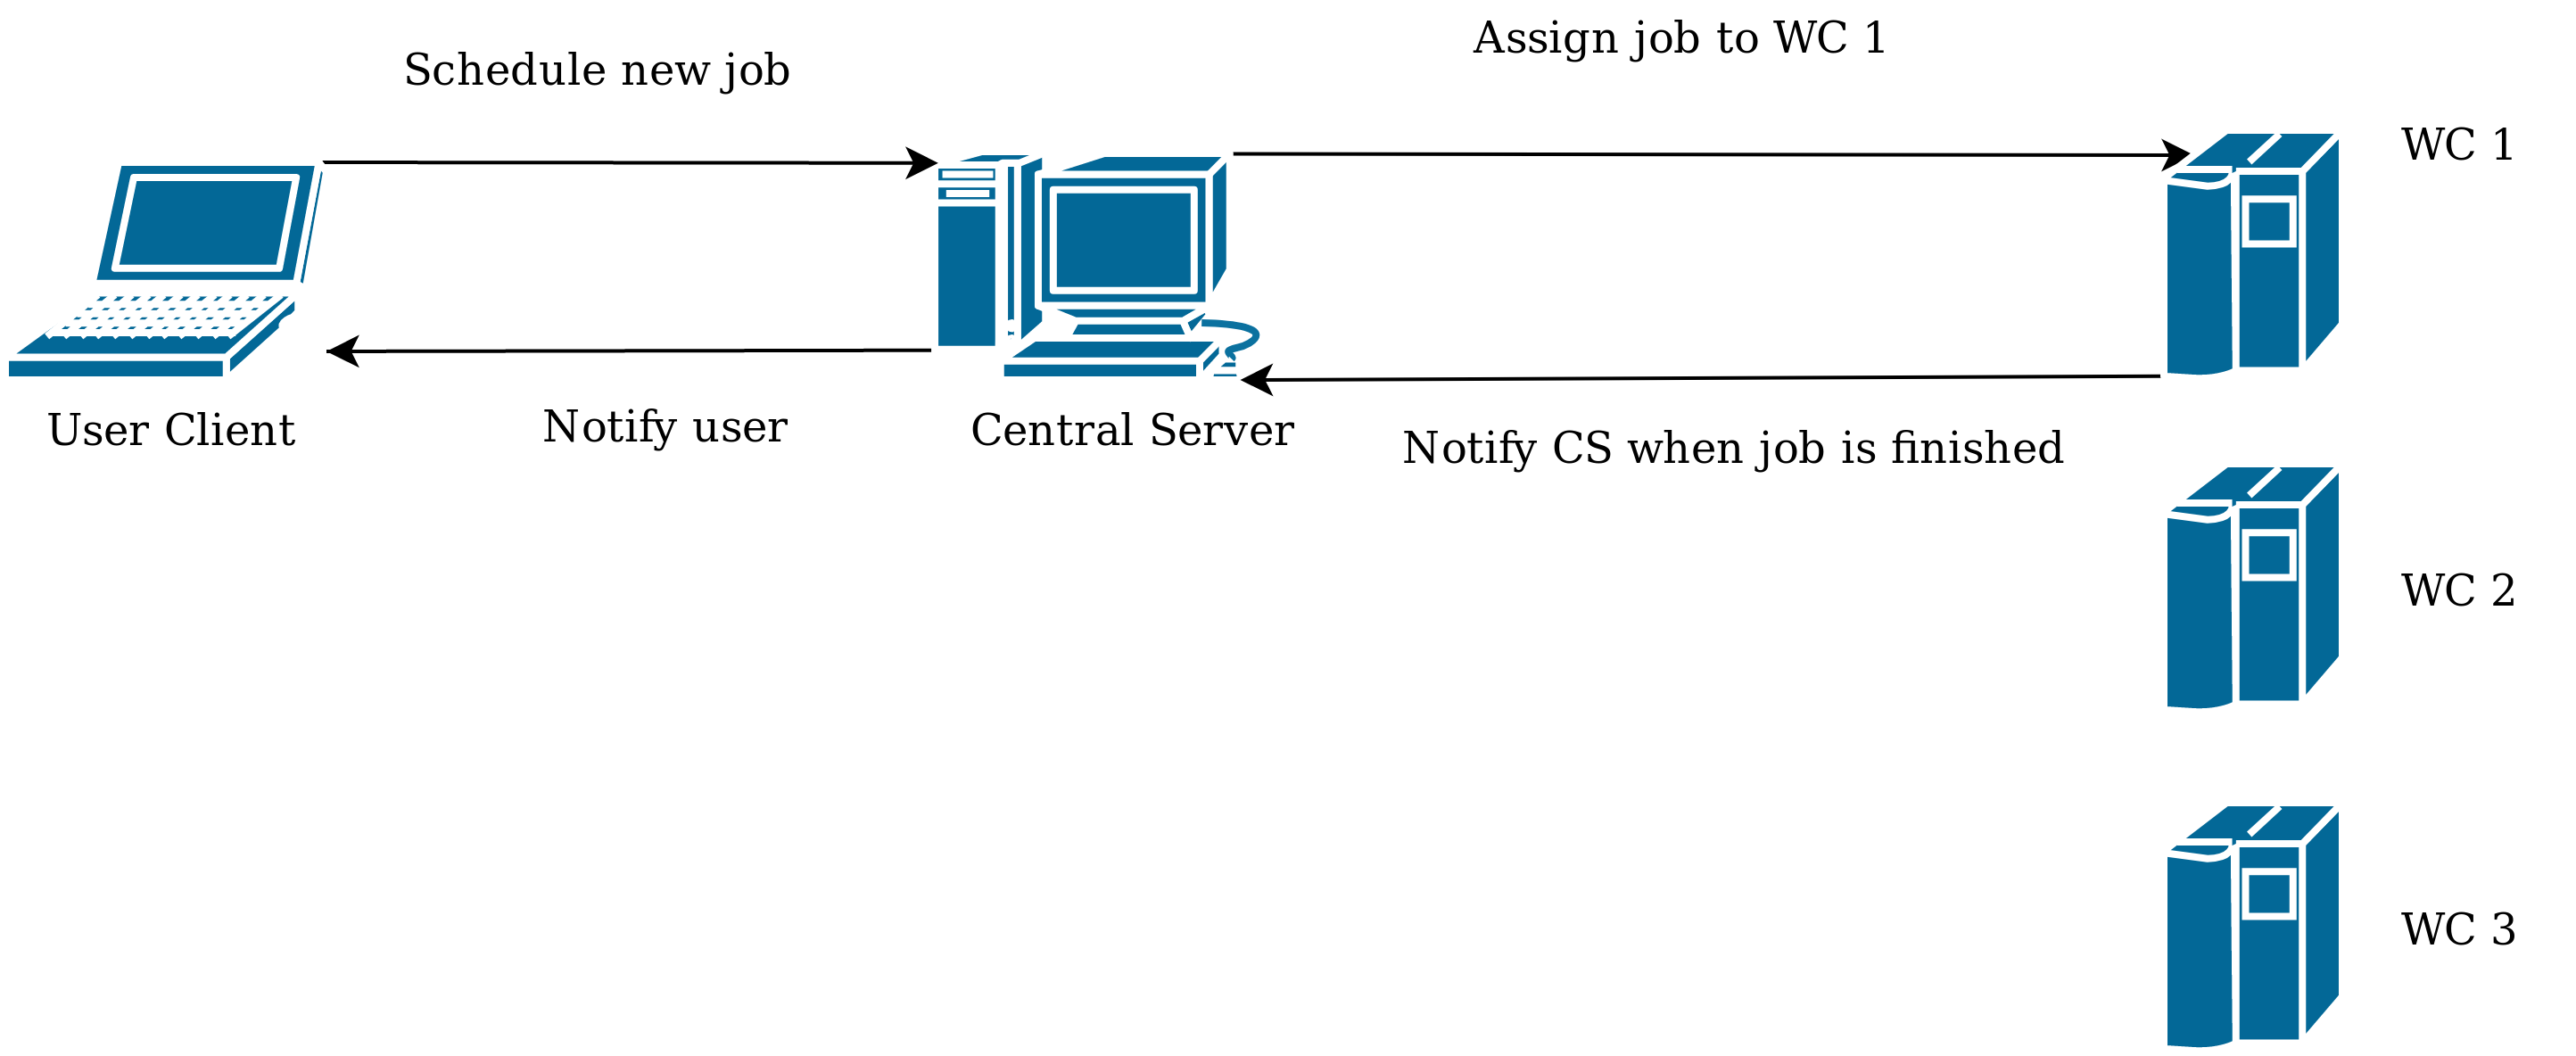
\includegraphics[width=\linewidth]{./system/systemmodel/images/schedulejob.png}
  \label{new-job}
  \caption{This diagram depicts how a user schedules a job, which the CS distributes to WC 1.
  In that case CS knows that there are enough resurces on WC 1 to execute users job.
  At the end the CS notifies the user that the job has finished.}
\end{figure}

\begin{figure}[H]
  \subsubsection{Access a job}
  \centering
  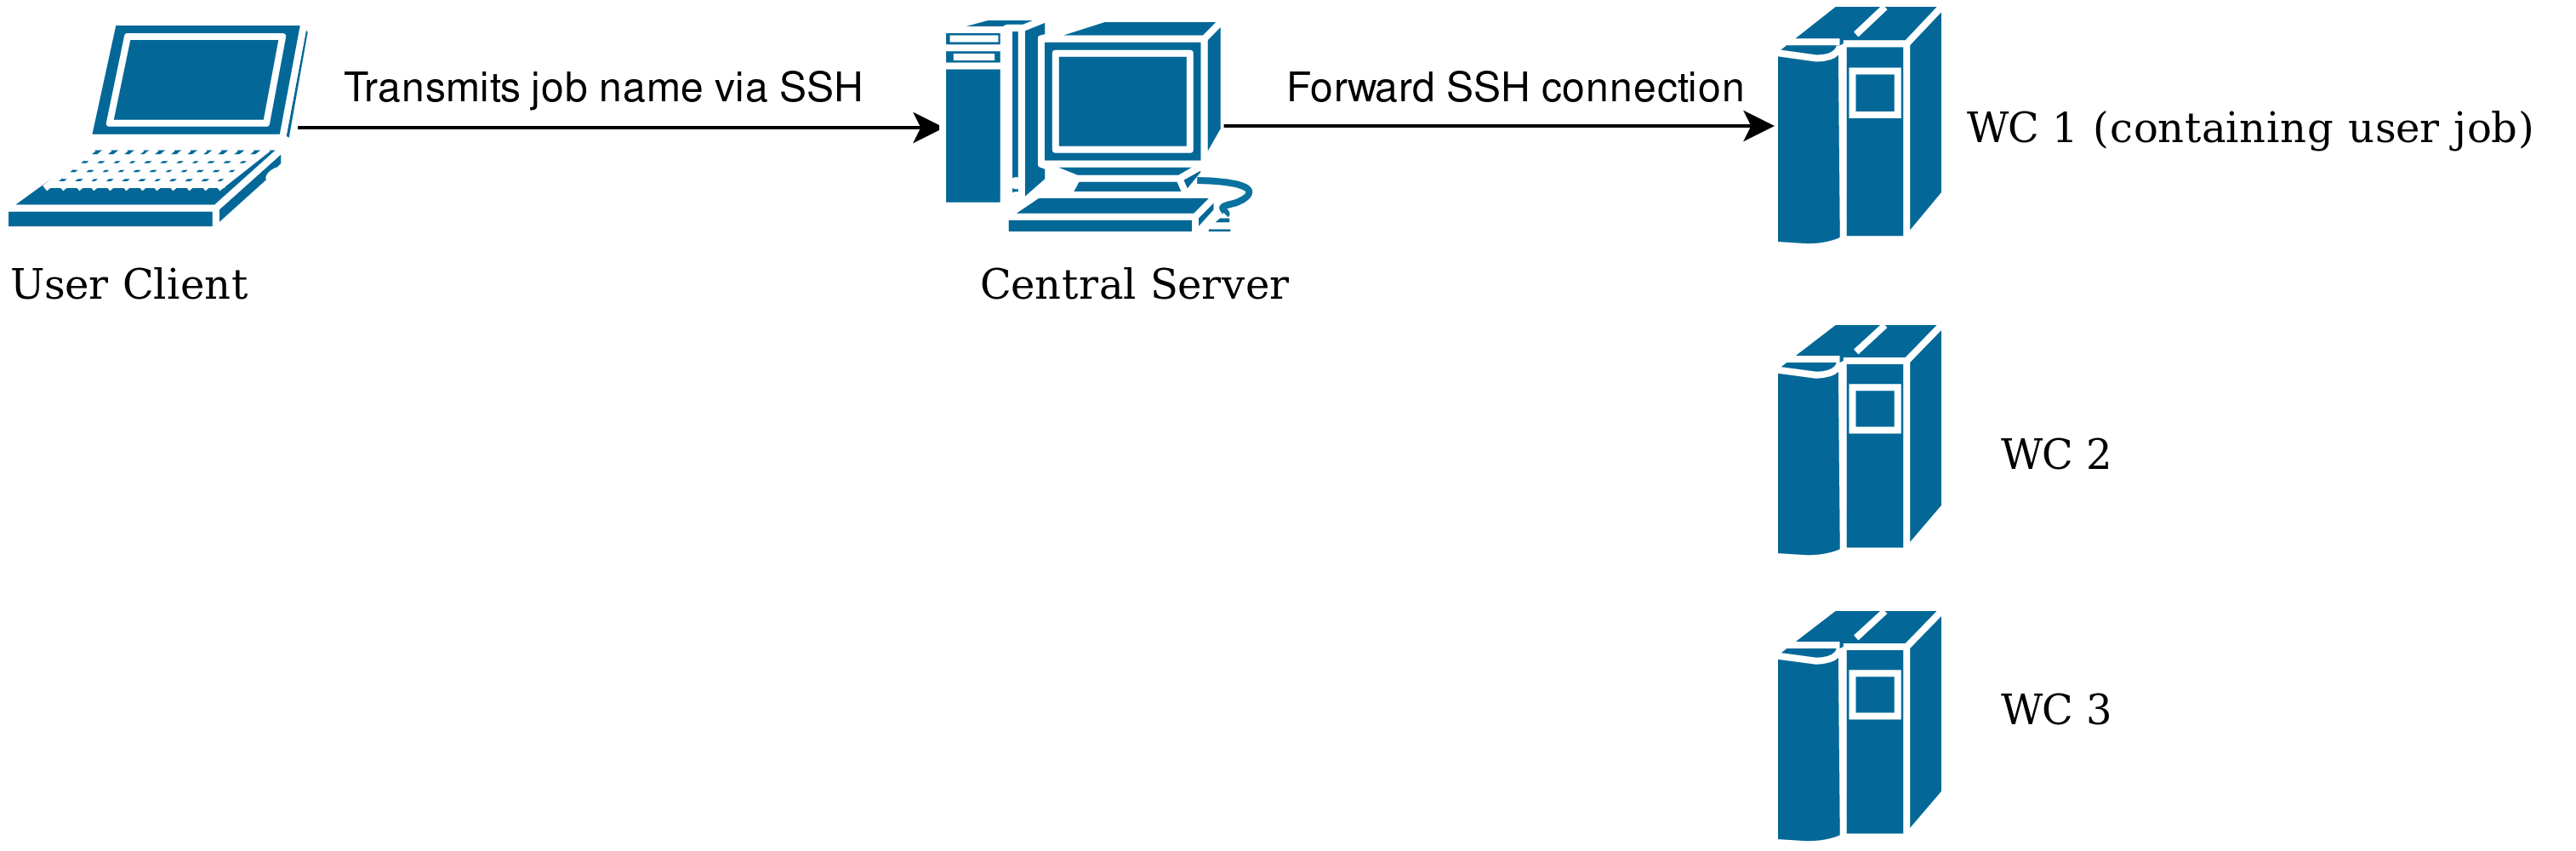
\includegraphics[width=\linewidth]{./system/systemmodel/images/accessjob.png}
  \label{access-job}
  \caption{This diagram depicts how a user accesses his job.
  The user has a job on one of the work machines that he wants to connect to.
  The user does not establish a direct connection with the WC.
  The user establishes an SSH connection to the server.
  This connection authenticates the user.
  It is also used to transmit the name of the job that the user wants to connect to.
  The server looks up which work machine the user's job is located on and forwards the SSH connection to that work machine.
  Finally, the SSH connection to the work machine is forwarded to the container with the user's job.}
\end{figure}

\begin{figure}[H]
  \subsubsection{Get statistics}
  \centering
  
\includegraphics[width=0.5\linewidth]{./system/systemmodel/images/statistics.png}
  \label{statistics}
  \caption{This diagram depicts how a user accesses the statistics saved on the server.}
\end{figure}
